\subsection{UI Design}

After researching upon several scenarios and storylines, we decided to create prototype of the UI first which would be highly flexible to fit any scenario or story. Our final UI is adapted from the prototype shown in Figure \ref{fig:uidesignprototype}.


\begin{figure}[H]
    \centering
    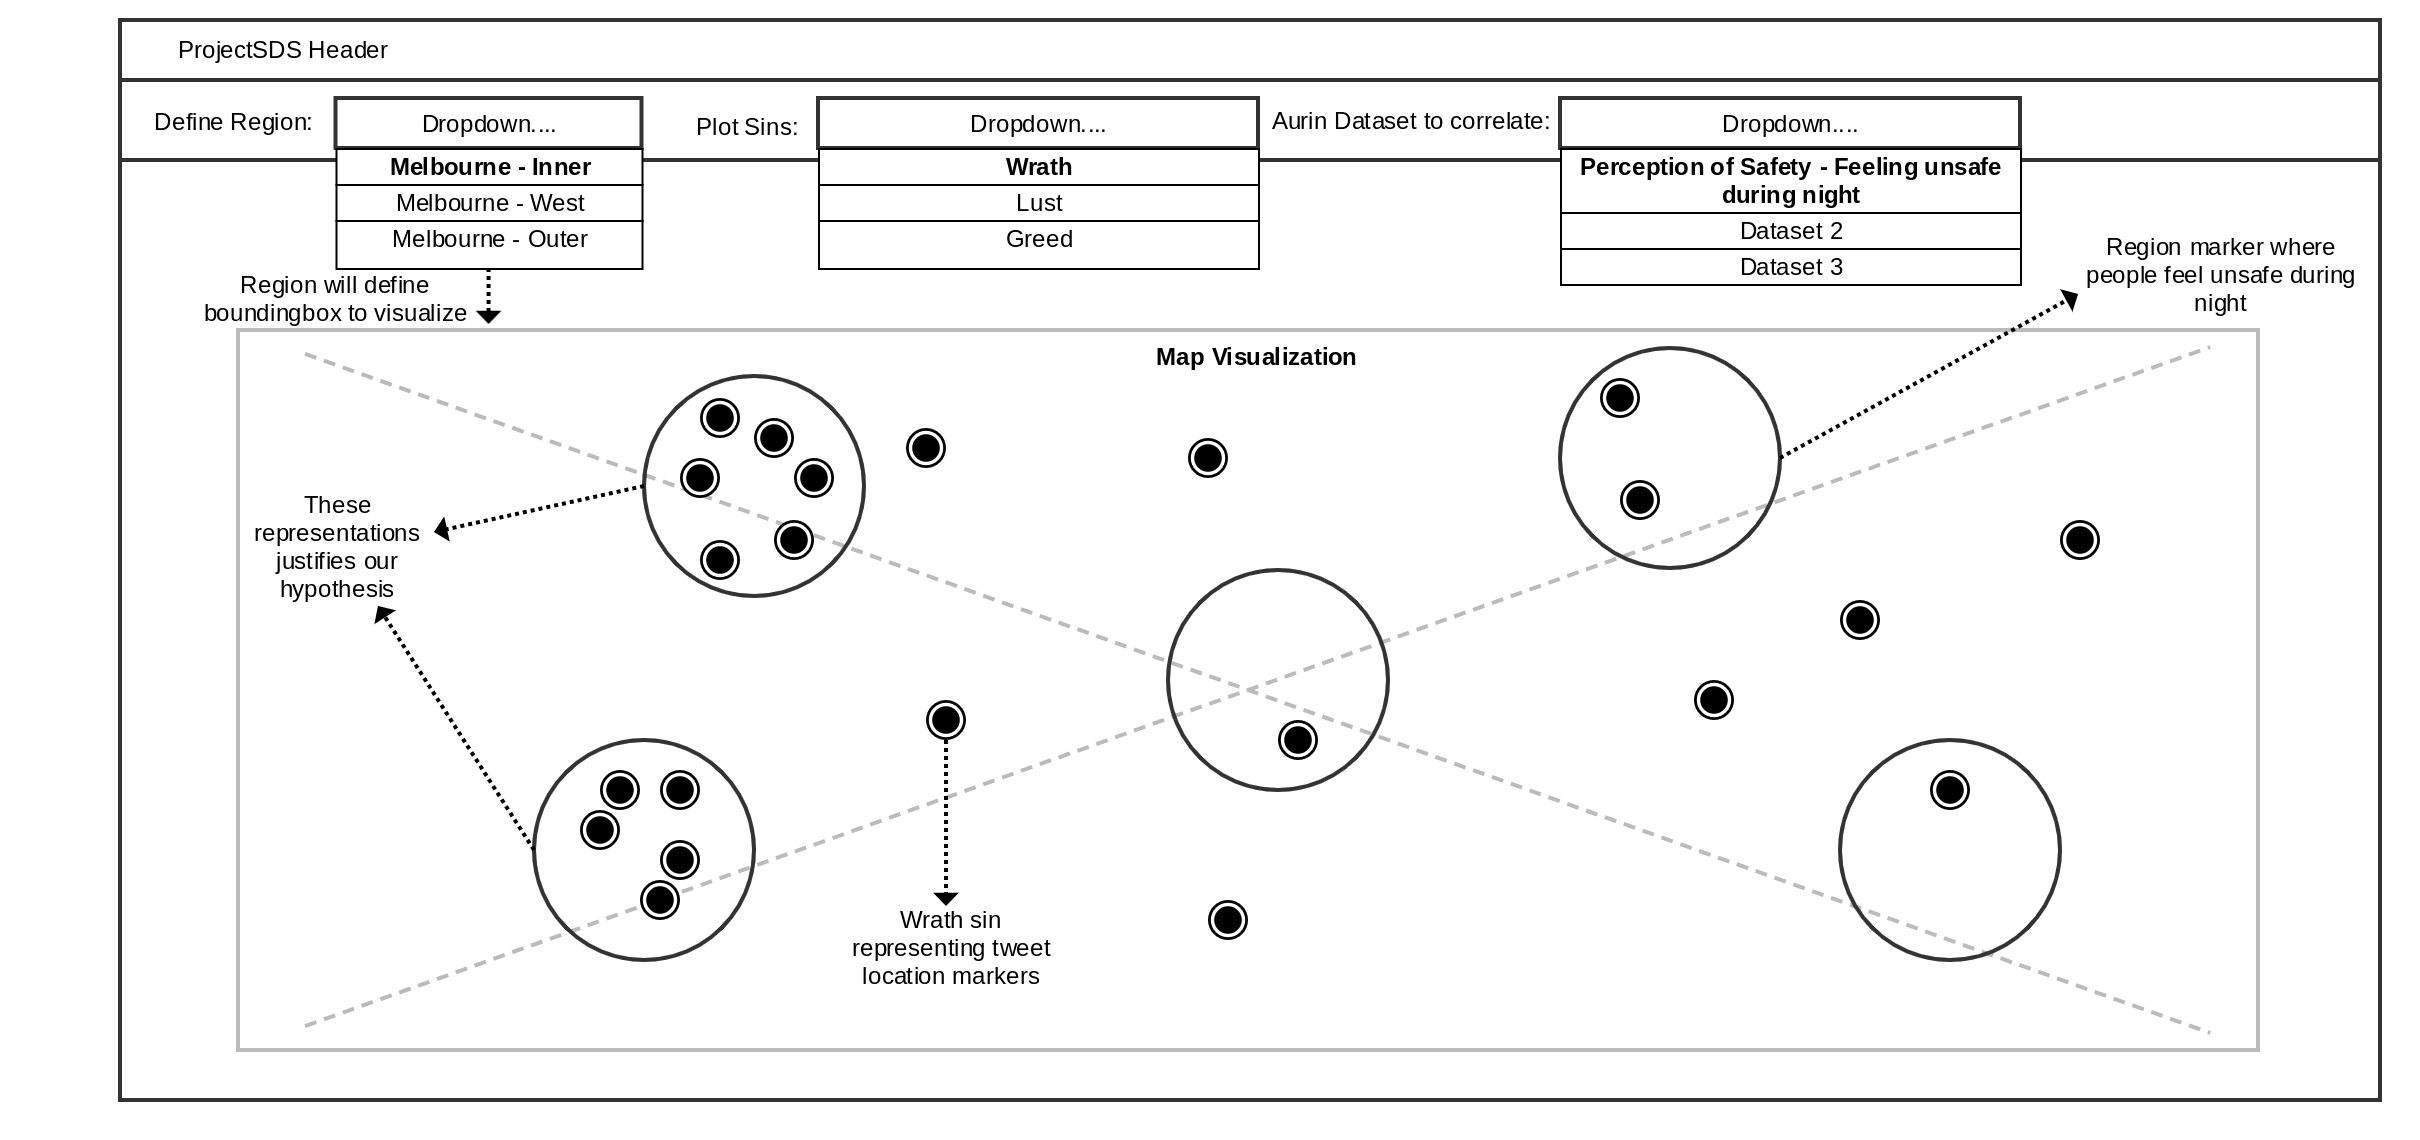
\includegraphics[width=16cm,keepaspectratio=true]{images/uiarchitecture.png}
    \caption{UI Design Prototype}
    \label{fig:uidesignprototype}
\end{figure}

The idea of the UI design is to visualize correlation between AURIN dataset and tweets found based on the sin for certain region. We were thinking of providing basic region filteration which will automatically select the area on the map. After that, user can choose one of the sins upon which tweets will be filtered. As soon as the user chooses sins for filteration, \texttt{black dots} markers will start to show on the map. This is then followed by the selection of AURIN data for correlation which creates \texttt{circle} on the map. 

This model is based on the assumption that - if we are able to find large number of tweets in certain region which is based on some sin and it is in correlation with the AURIN data, then we have proved our hypothesis.